% ============================================================
% poster.tex:Academic Recruiting Poster
% "Stochastic Attention via Langevin Dynamics on the Modern Hopfield Energy"
% Alswaidan & Varner, Cornell University
%
% Compile with: pdflatex poster.tex
% Figures referenced from ../paper/figs/
% Logo from  logo/cornell_logo.pdf
% ============================================================

\documentclass[final]{beamer}

% --- Poster size: 36" x 48" portrait (91.44 cm x 121.92 cm) ---
\usepackage[orientation=portrait, size=custom,
            width=91.44, height=121.92, scale=1.0]{beamerposter}

\usepackage[utf8]{inputenc}
\usepackage[T1]{fontenc}
\usepackage{lmodern}
\usepackage{graphicx}
\usepackage{booktabs}
\usepackage{amsmath,amssymb}
\usepackage{xcolor}
\usepackage{tikz}
\usepackage{microtype}
\usepackage{array}
\usepackage{ragged2e}
\usepackage{enumitem}
\usepackage[nolinks]{qrcode}

% ============================================================
% Cornell color palette
% ============================================================
\definecolor{CornellRed}{RGB}{179,27,27}
\definecolor{CornellLightGray}{RGB}{247,247,247}
\definecolor{CornellMidGray}{RGB}{200,200,200}
\definecolor{CornellDarkGray}{RGB}{70,70,70}

% ============================================================
% Beamer theme
% ============================================================
\usetheme{default}
\setbeamertemplate{navigation symbols}{}

\setbeamercolor{background canvas}{bg=white}
\setbeamercolor{block title}{fg=white, bg=black}
\setbeamercolor{block body}{fg=black, bg=white}
\setbeamercolor{block alerted title}{fg=white, bg=CornellDarkGray}
\setbeamercolor{block alerted body}{fg=black, bg=white}

\setbeamerfont{block title}{size=\Large, series=\bfseries}
\setbeamerfont{block body}{size=\large}

% Compact block templates:no box on title, just bold black text
\setbeamertemplate{block begin}{%
  \vskip6pt
  {\usebeamerfont{block title}\color{black}\insertblocktitle}\\[-2pt]
  \textcolor{CornellMidGray}{\rule{\linewidth}{0.8pt}}
  \begin{beamercolorbox}[rounded=true,shadow=false,colsep*=0.5ex,vmode,
      leftskip=0.3em,rightskip=0.3em]{block body}%
    \usebeamerfont{block body}\vskip4pt%
}
\setbeamertemplate{block end}{%
  \vskip4pt\end{beamercolorbox}\vskip6pt%
}

\setbeamertemplate{block alerted begin}{%
  \vskip6pt
  {\usebeamerfont{block title}\color{black}\insertblocktitle}\\[-2pt]
  \textcolor{CornellMidGray}{\rule{\linewidth}{0.8pt}}
  \begin{beamercolorbox}[rounded=true,shadow=false,colsep*=0.5ex,vmode,
      leftskip=0.3em,rightskip=0.3em]{block alerted body}%
    \usebeamerfont{block body}\vskip4pt%
}
\setbeamertemplate{block alerted end}{%
  \vskip4pt\end{beamercolorbox}\vskip6pt%
}

% ============================================================
\begin{document}
\begin{frame}[t]

% ============================================================
% HEADER: Logo | Title | Authors (left-justified, aligned with logo)
% ============================================================
\vspace*{4pt}
\begin{columns}[c, totalwidth=\linewidth]

  \begin{column}{0.10\linewidth}
    \centering
    \includegraphics[width=0.88\linewidth]{logo/cornell_logo.pdf}
  \end{column}

  \begin{column}{0.78\linewidth}
    \raggedright
    {\color{black}\bfseries\fontsize{56}{64}\selectfont
      Stochastic Attention via Langevin Dynamics on the Modern Hopfield Energy}\\[8pt]
    {\fontsize{34}{40}\selectfont
      Abdulrahman Alswaidan \& Jeffrey D.\ Varner}\\[6pt]
    {\fontsize{26}{32}\selectfont\color{black}
      R.F.\ Smith School of Chemical and Biomolecular Engineering, Cornell University
      \quad \texttt{\{aa2725, jdv27\}@cornell.edu}}
  \end{column}

  \begin{column}{0.10\linewidth}
    \centering
    \qrcode[height=3.5cm]{https://varnerlab.org}\\[4pt]
    {\fontsize{18}{22}\selectfont\color{black} varnerlab.org}
  \end{column}

\end{columns}

\vspace{16pt}
\textcolor{black}{\rule{\linewidth}{3pt}}
\vspace{2pt}

% ============================================================
% BODY:two equal columns
% ============================================================
\begin{columns}[t, totalwidth=\linewidth]

% ################################################################
% LEFT COLUMN
% ################################################################
\begin{column}{0.475\linewidth}

% -----------------------------------------------------------
\begin{block}{Motivation}
% -----------------------------------------------------------
\justifying
Attention heads are deterministic: the same query always returns the same softmax-weighted memory average.
Yet many tasks require \emph{generating} novel, plausible patterns from structured memory.

We show that the gradient of the \textbf{modern Hopfield energy} is exactly the identity minus the attention map, and that applying \textbf{Langevin dynamics} to this energy yields \emph{stochastic attention}: a \textbf{training-free sampler} controlled by a single inverse temperature $\beta$.

\vspace{4pt}
\begin{center}
  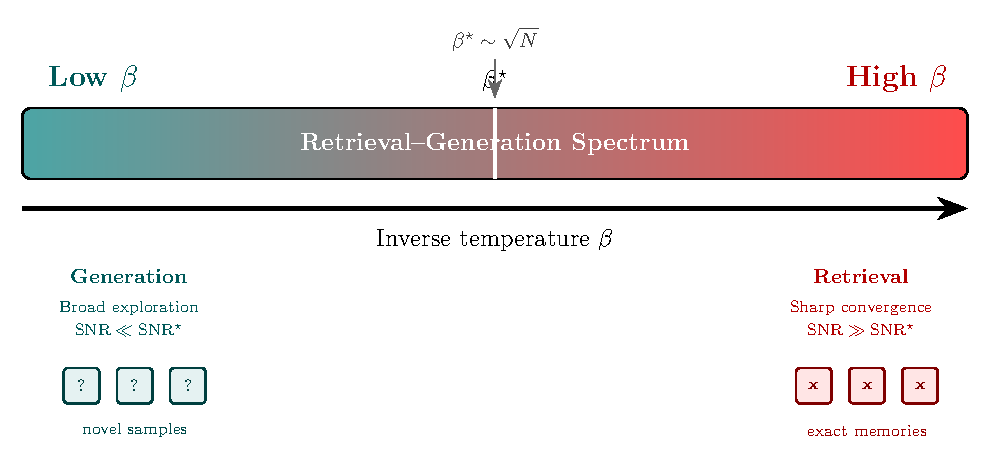
\includegraphics[width=0.96\linewidth]{figs/Fig-Beta-Spectrum.pdf}
\end{center}

\vspace{2pt}
The critical temperature $\beta^{\star}$ marks the retrieval--generation boundary, identified analytically via an entropy inflection condition: $\beta^{\star}\!\sim\!\sqrt{d}$ for random unit-norm memories.
\textbf{No score network, no training loop, no contrastive objective}:the score is the attention map itself.
\end{block}

% -----------------------------------------------------------
\begin{block}{Method: Stochastic Attention Update}
% -----------------------------------------------------------
$\mathbf{X} = [\mathbf{m}_1,\dots,\mathbf{m}_K]\!\in\!\mathbb{R}^{N\times K}$ stores $K$ patterns.
To generate, we sample from $p_\beta(\boldsymbol{\xi})\!\propto\!\exp(-\beta E(\boldsymbol{\xi}))$.

\vspace{6pt}
The ULA turns any smooth energy $U$ into a sampler:
\[
  \boldsymbol{\xi}_{t+1} = \boldsymbol{\xi}_t - \tilde\alpha\,\nabla U(\boldsymbol{\xi}_t) + \sqrt{2\tilde\alpha}\;\boldsymbol{\epsilon}_t,
  \qquad \boldsymbol{\epsilon}_t \sim \mathcal{N}(\mathbf{0},\mathbf{I}).
\]

The gradient of the modern Hopfield energy is exactly the attention residual:
\[
  \nabla E(\boldsymbol{\xi})
  = \boldsymbol{\xi} - \underbrace{\mathbf{X}\,\mathrm{softmax}(\beta\,\mathbf{X}^\top\boldsymbol{\xi})}_{\mathbf{T}(\boldsymbol{\xi})\;=\;\text{softmax attention map}}.
\]

Substituting $\nabla E$ into the ULA (with $U = \beta E$, $\tilde\alpha = \alpha/\beta$):

\begin{center}
  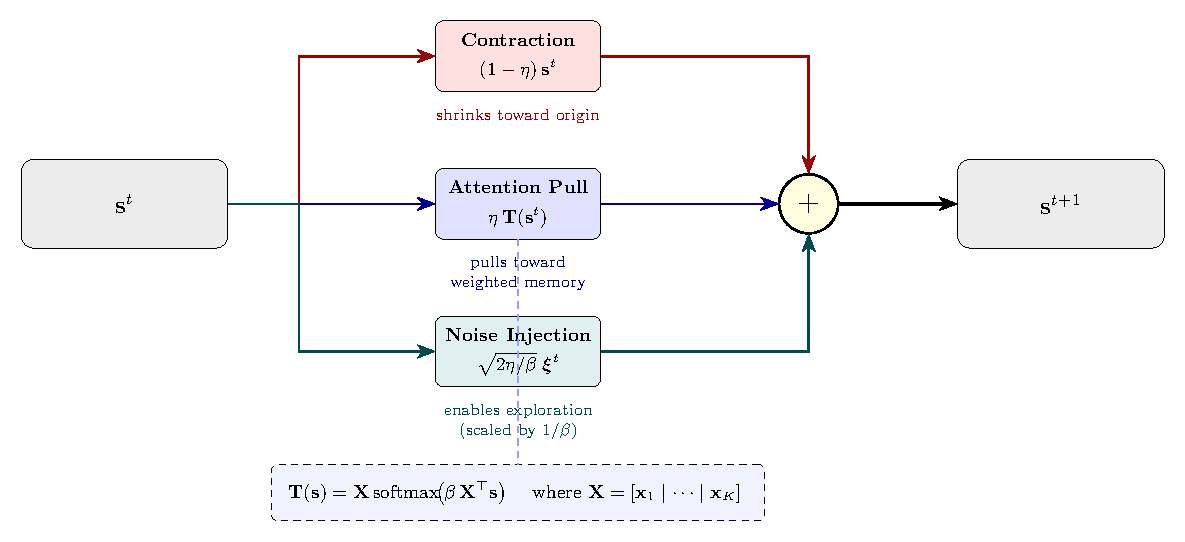
\includegraphics[width=0.96\linewidth]{figs/Fig-Stochastic-Attention-Update.pdf}
\end{center}
\[
  \boldsymbol{\xi}_{t+1}
  = \underbrace{(1-\alpha)\,\boldsymbol{\xi}_t}_{\text{contraction}}
  + \underbrace{\alpha\,\mathbf{X}\,\mathrm{softmax}(\beta\,\mathbf{X}^\top\!\boldsymbol{\xi}_t)}_{\text{attention pull to memories}}
  + \underbrace{\sqrt{\tfrac{2\alpha}{\beta}}\;\boldsymbol{\epsilon}_t}_{\text{Gaussian noise}}
\]

\vspace{2pt}
\begin{itemize}[leftmargin=1.2em, itemsep=1pt]
  \item \textbf{Step cost:} $\mathcal{O}(dK)$: same as one attention head; no training required.
  \item \textbf{Convergence:} $W_2$-geometric in the convex regime ($\beta\sigma_{\max}^2 < 2$); MALA acceptance $= 99.2\%$ at $\alpha\!=\!0.01$ confirms negligible discretization bias.
  \item \textbf{Temperature selection:} $\beta^*$ via entropy inflection $d^2H/d\beta^2\!=\!0$; scales as $\beta^*\!\sim\!\sqrt{d}$.
\end{itemize}
\end{block}

% -----------------------------------------------------------
\begin{block}{Experiment 1:Phase Behavior \& Convergence (Synthetic)}
% -----------------------------------------------------------
Does $\beta$ really act as a continuous order parameter between generation and retrieval, and does the sampler converge to the correct Boltzmann target? If the theory is right, we should see a smooth sigmoidal transition in both cosine similarity and attention entropy, with the inflection landing near the predicted $\beta^*\!\sim\!\sqrt{d}$.

\vspace{4pt}
\begin{center}
  
\includegraphics[width=0.96\linewidth]{../paper/figs/Fig_experiment-combined.pdf}
\end{center}
{\small
\textbf{(a)} $d\!=\!64$, $K\!=\!16$.
Cosine similarity (blue) and scaled entropy (coral) exhibit a smooth sigmoidal transition centered at $\beta\!\approx\!5$--$10$ (gold band), consistent with the predicted $\beta^*\!\sim\!\sqrt{d}$.\\[2pt]
\textbf{(b)} $d\!=\!8$, $K\!=\!4$, $\beta\!=\!5$.
Eight independent chains (gray) converge to a long-run reference (coral); KS statistic confirms the correct Boltzmann target.
}
\end{block}

\end{column}
% end LEFT COLUMN

% ################################################################
% RIGHT COLUMN
% ################################################################
\begin{column}{0.475\linewidth}

% -----------------------------------------------------------
\begin{block}{Experiment 2:MNIST Image Generation ($K=100$, $d=784$)}
% -----------------------------------------------------------
Can stochastic attention generate structured, recognizable images from a small memory, and how does it compare to learned generative models on the same data?

\vspace{4pt}
$K\!=\!100$ images of digit ``3''; 30 independent chains; 150 generated samples.
$\beta\!=\!2000$ (retrieval) and $\beta\!=\!200$ (generation, near $\beta^*$).

\vspace{6pt}
\begin{columns}[t, totalwidth=\linewidth]
  \begin{column}{0.48\linewidth}
    \centering
    {\small
    \setlength{\tabcolsep}{3pt}
    \begin{tabular}{@{}lccc@{}}
    \toprule
    \textbf{Method} & \textbf{Nov.}$\uparrow$ & \textbf{Div.}$\uparrow$ & \textbf{Energy}$\downarrow$ \\
    \midrule
    Bootstrap            & $0.000$ & $0.459$ & $-0.500$ \\
    Gaussian perturb.    & $0.004$ & $0.450$ & $-0.496$ \\
    Convex combo         & $0.092$ & $0.008$ & $-0.399$ \\
    GMM-PCA              & $0.198$ & $0.419$ & $-0.303$ \\
    VAE (latent $=8$)    & $0.214$ & $0.441$ & $-0.286$ \\
    DDPM\textsuperscript{\dag} & $0.938$ & $0.991$ & $+0.44$ \\
    MALA ($\beta\!=\!2000$)   & $0.151$ & $0.598$ & $-0.305$ \\
    SA ($\beta\!=\!2000$) & $0.152$ & $0.600$ & $-0.303$ \\
    \textbf{SA ($\beta\!=\!200$)} & $\mathbf{0.548}$ & $\mathbf{0.885}$ & $+1.467$ \\
    \bottomrule
    \end{tabular}
    }
    \vspace{4pt}

    {\small\textsuperscript{\dag}DDPM generates isotropic noise despite 5,000 training epochs.}
  \end{column}
  \begin{column}{0.50\linewidth}
    \centering
    \begin{tabular}{@{}cc@{}}
      \includegraphics[width=0.47\linewidth]{../code/figs/Fig_mnist_grid_sa_digit3.png} &
      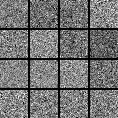
\includegraphics[width=0.47\linewidth]{../code/figs/Fig_mnist_grid_ddpm_digit3.png} \\[2pt]
      {\small \textbf{SA} ($\beta\!=\!2000$)} & {\small \textbf{DDPM}}
    \end{tabular}
  \end{column}
\end{columns}

\vspace{4pt}
SA at $\beta\!=\!200$ achieves $\mathbf{2.6\times}$ the novelty and $\mathbf{2.0\times}$ the diversity of the VAE, while matching the Metropolis-corrected MALA gold standard. Crucially, DDPM fails entirely despite 5,000 training epochs — the training-free score function provides a structural advantage that a learned model cannot recover from only 100 examples.
\end{block}

% -----------------------------------------------------------
\begin{block}{Experiment 3:Protein Sequence Generation (Pfam RRM, $K=68$, $d=59$)}
% -----------------------------------------------------------
Does the training-free score function preserve domain-level biological fidelity when generating novel sequences, something learned models struggle with at small $K$?

\vspace{4pt}
68 aligned RRM sequences; one-hot encoded, PCA-reduced (95\% variance).
Entropy inflection gives $\beta^*\!=\!3.85$ (half the random-pattern prediction $\sqrt{d}\!=\!7.68$; conserved residues increase effective similarity variance).

\vspace{4pt}
\begin{columns}[c, totalwidth=\linewidth]
  \begin{column}{0.50\linewidth}
    \centering
    \setlength{\tabcolsep}{5pt}
    \begin{tabular}{@{}lcccc@{}}
    \toprule
    \textbf{Method} & \textbf{Nov.}$\uparrow$ & \textbf{Div.}$\uparrow$ & \textbf{SeqID} & \textbf{KL}$\downarrow$ \\
    \midrule
    Bootstrap         & $0.000$ & $1.000$ & $0.645$ & $0.133$ \\
    VAE               & $0.621$ & $0.834$ & $0.532$ & $0.416$ \\
    SA (retrieval)    & $0.243$ & $0.991$ & $0.616$ & $0.107$ \\
    \textbf{SA (gen.)}& $\mathbf{0.623}$ & $\mathbf{1.001}$ & $0.538$ & $\mathbf{0.060}$ \\
    \bottomrule
    \end{tabular}
  \end{column}
  \begin{column}{0.48\linewidth}
    \centering
    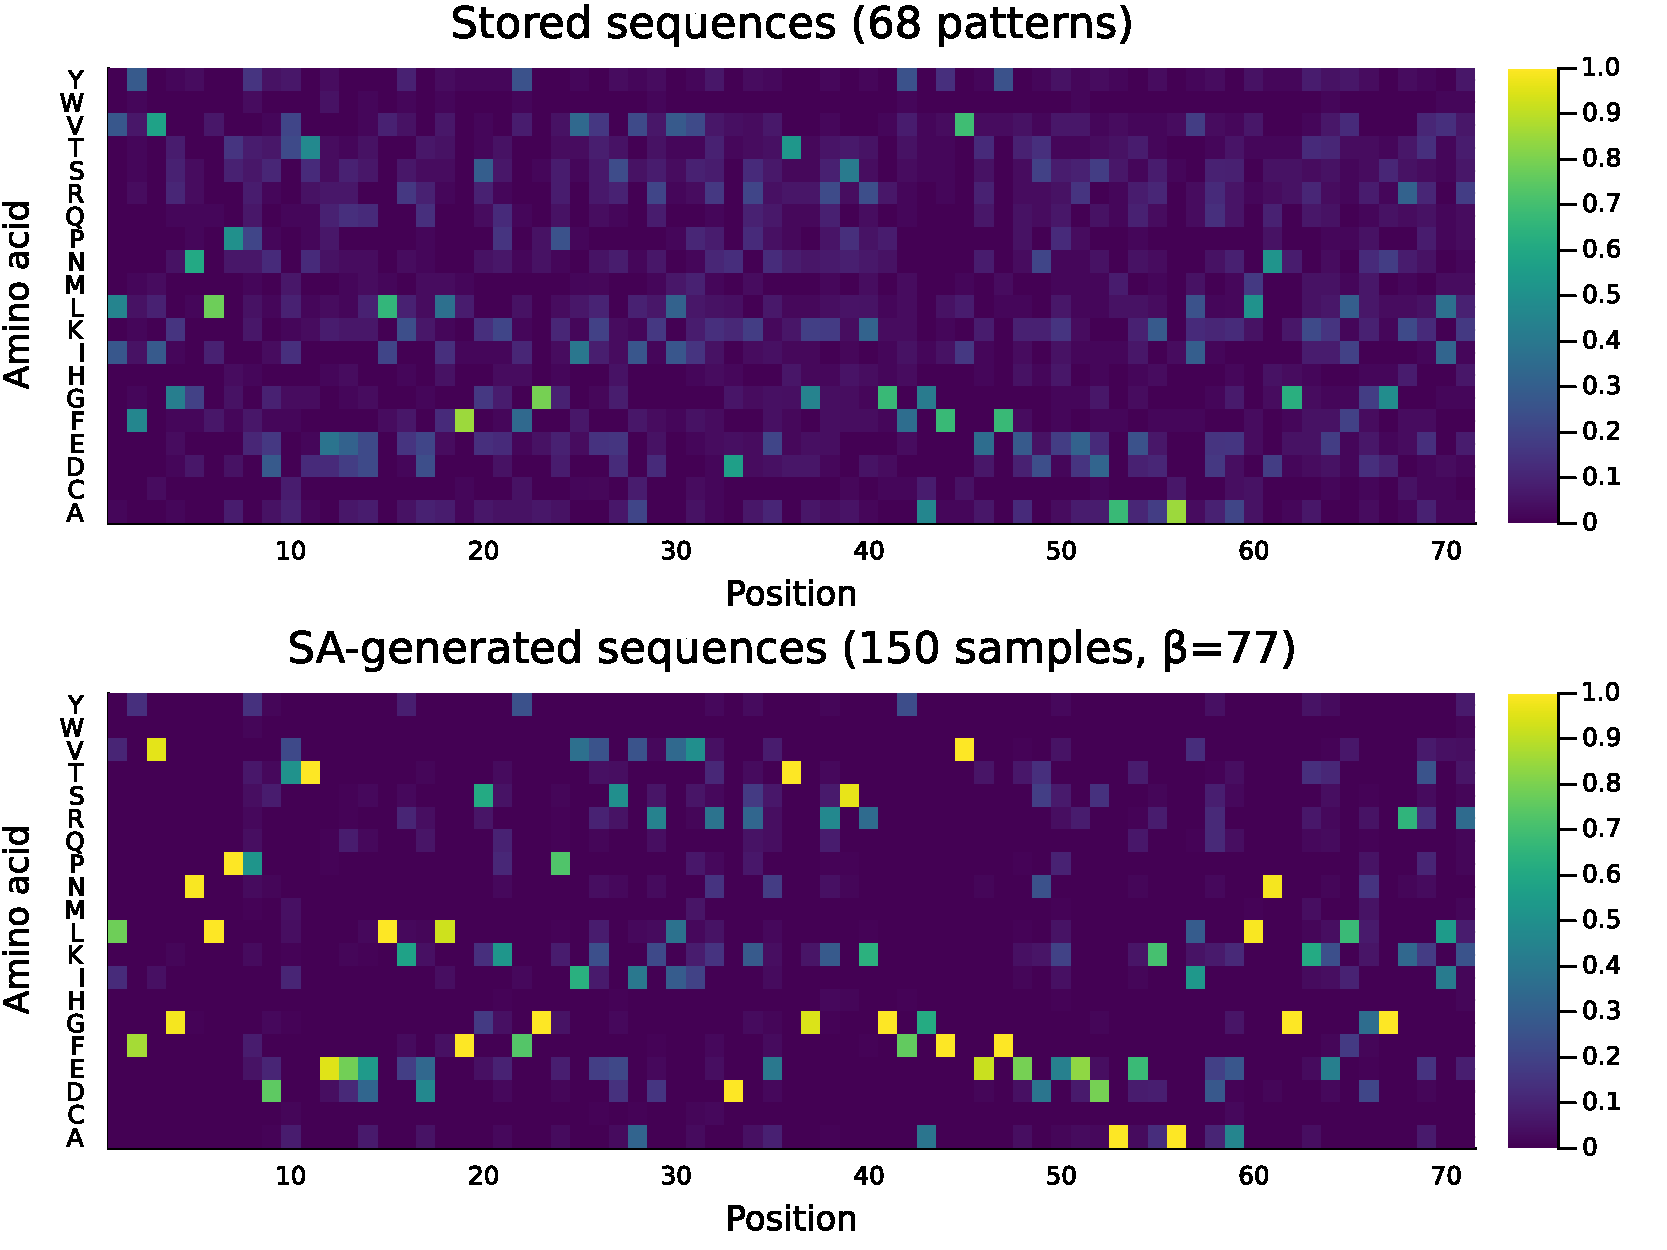
\includegraphics[width=\linewidth]{../paper/figs/Fig_protein_aa_frequencies.pdf}
    {\small Stored (top) vs.\ SA-generated (bottom) amino acid frequencies.}
  \end{column}
\end{columns}

\vspace{4pt}
SA matches the VAE on novelty while achieving $\mathbf{6.9\times}$ lower amino acid composition divergence (KL $= 0.060$ vs.\ $0.416$). Because the Langevin gradient is recomputed from the stored sequences at every step, it continuously steers samples back toward the family's compositional profile — fidelity the VAE loses when trained on only 68 sequences.
\end{block}

% -----------------------------------------------------------
\begin{block}{Experiment 4:Scaling to Face Images --- Simpsons ($d=4{,}096$)}
% -----------------------------------------------------------
Does SA still work when we scale to high-dimensional image data, and does the $\beta^*\!\sim\!\sqrt{d}$ rule remain a reliable guide for temperature selection?

\vspace{4pt}
\begin{columns}[c, totalwidth=\linewidth]
  \begin{column}{0.48\linewidth}
    \centering
    
\includegraphics[width=\linewidth]{../code/figs/Fig_simpsons_grid_sa.png}
    {\small SA-generated faces ($\beta\!=\!10{,}000$, retrieval regime).}
  \end{column}
  \begin{column}{0.50\linewidth}
    \justifying
    $64\!\times\!64$ grayscale Simpsons character images ($d\!=\!4{,}096$).
    The SNR rule prescribes $\beta^*\!\sim\!\sqrt{4096}\!=\!64$; we run at $\beta\!=\!10{,}000$ (well inside retrieval).

    \vspace{8pt}
    SA achieves novelty $0.159\!\pm\!0.000$ and diversity $0.293\!\pm\!0.001$, with \textbf{identical method ranking to MNIST} across a $\mathbf{5.2\times}$ increase in dimension.
    The SNR selection rule transfers directly from 784 to 4,096 dimensions with no tuning.
  \end{column}
\end{columns}
\end{block}

% -----------------------------------------------------------
\begin{alertblock}{Limitations \& Future Work}
% -----------------------------------------------------------
\begin{itemize}[leftmargin=1.2em, itemsep=2pt]
  \item \textbf{ULA bias} scales with step size $\alpha$; MALA (with Metropolis correction) is preferred at larger $\alpha$.
  \item \textbf{Inter-basin mixing} at high $\beta$ is exponentially slow; the multi-chain protocol provides a practical workaround, but quantitative scaling laws remain open.
  \item \textbf{Fixed memory:} $\mathbf{X}$ must be known at sampling time; streaming or latent memory settings require extension.
  \item \textbf{Generation fidelity} at high temperature yields structured interpolations rather than crisp samples; operating near $\beta^*$ improves quality.
  \item \textbf{Future:} multi-head attention, hierarchical memories, retrieval-augmented generation, in-context learning.
\end{itemize}
\end{alertblock}

\end{column}
% end RIGHT COLUMN

\end{columns}

% ============================================================
% FOOTER
% ============================================================
\vfill
\textcolor{CornellMidGray}{\rule{\linewidth}{2pt}}
\vspace{4pt}
\qrcode[height=6cm]{https://github.com/varnerlab/stochastic-attention-study-paper}\\[4pt]
{\fontsize{18}{22}\selectfont\color{black} github.com/varnerlab/stochastic-attention-study-paper}

\end{frame}
\end{document}
